\input{configuration}

\def\ojoin{\setbox0=\hbox{$\bowtie$}%
  \rule[-.02ex]{.25em}{.4pt}\llap{\rule[\ht0]{.25em}{.4pt}}}
\def\leftouterjoin{\mathbin{\ojoin\mkern-5.8mu\bowtie}}

\title{Tutorial 7 --- Data Mining and Transactions }

\author{Richard Wong \\ \small \texttt{rk2wong@edu.uwaterloo.ca}}
\institute{Department of Electrical and Computer Engineering \\
  University of Waterloo}
\date{\today}


\begin{document}

\begin{frame}
  \titlepage

\end{frame}


\begin{frame}
\frametitle{Exercise 7-1}

What is a data warehouse, and why is it useful to have one?

\end{frame}


\begin{frame}
\frametitle{Exercise 7-2}

Suppose we are trying to predict the value \textit{Wait}. \\
Between attributes \textit{Pat} and \textit{Type}, which is better to split a decision node on?

\begin{center}
  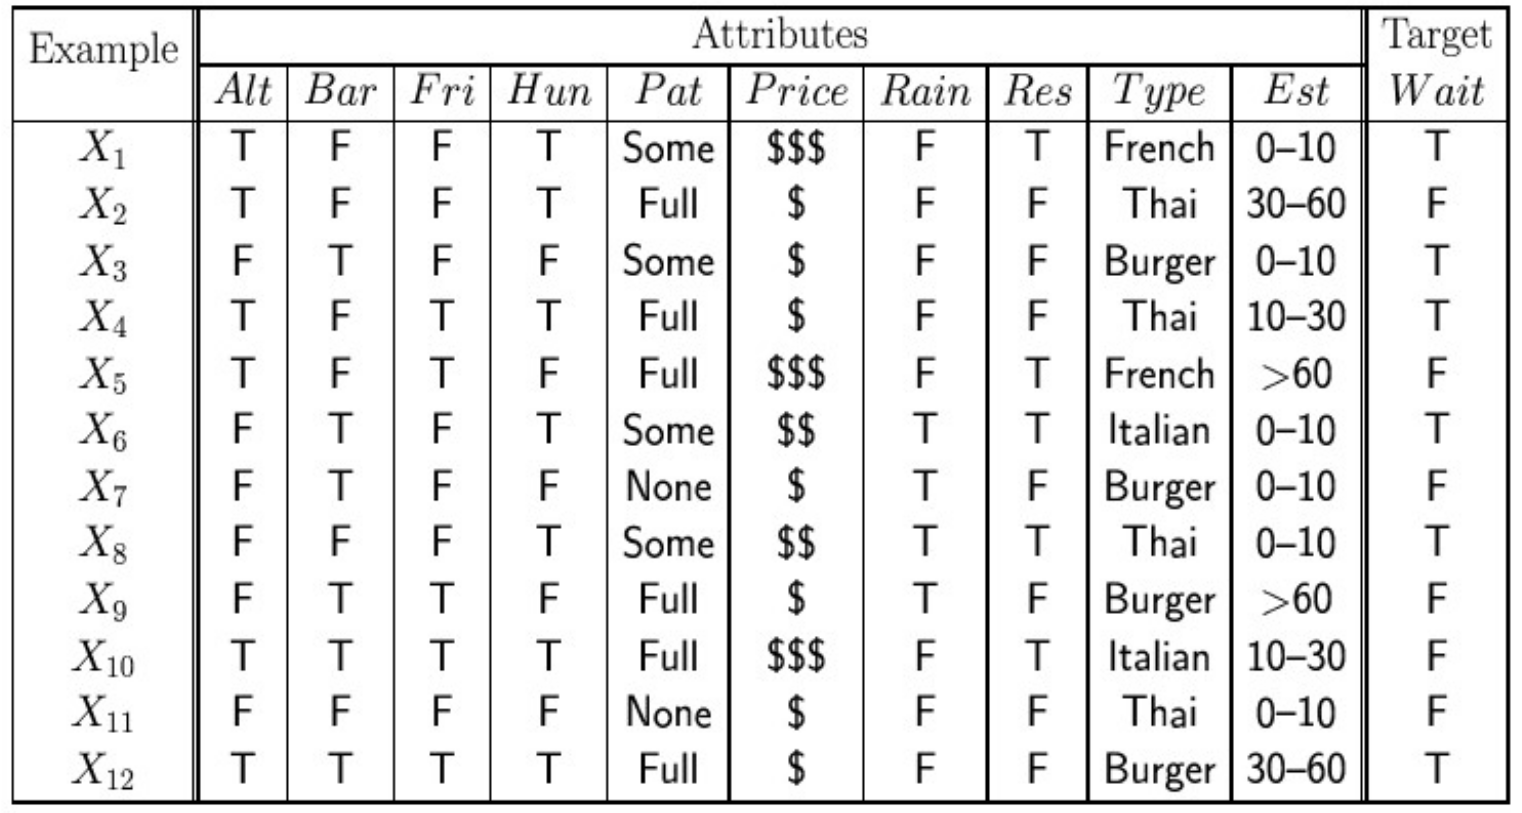
\includegraphics[width=0.9\textwidth]{images/decision_matrix.png}
\end{center}

\end{frame}


\begin{frame}
\frametitle{Exercise 7-3}

What are the ACID transaction properties, and what can a database do to ensure each one?

\end{frame}


\begin{frame}
\frametitle{Exercise 7-4}

Distinguish between the following:

\begin{enumerate}
  \item a serial schedule
  \item a serializable schedule
  \item a conflict-serializable schedule
\end{enumerate}

\end{frame}


\begin{frame}
\frametitle{Exercise 7-5}

Is the following schedule conflict-serializable? \\
If not, what can the database transaction manager do to make the schedule conflict-serializable?


\begin{center}
\begin{tabular}{ c c c c c c c }
  \hline
  T1 & r(x) & & w(y) & & & \\
  \hline
  T2 & & r(y) & & & r(x) & \\
  \hline
  T3 & & & & w(x) & & r(x) \\
  \hline
\end{tabular}
\end{center}

\end{frame}
\end{document}
